\documentclass[unicode,a4paper,10pt]{ltjsarticle}
% ---fonts---
\PassOptionsToPackage{quiet}{fontspec}
\usepackage{luatexja-fontspec}
\setmainfont{TeX Gyre Termes}
\setmainjfont[BoldFont = IPAGothic]{IPAMincho}
% \setmainjfont{Noto Sans CJK JP}
\setmathrm{Latin Modern Roman}

% ---Display \subsubsection at the Index
% \setcounter{tocdepth}{3}

% ---Setting about the geometry of the document----
% \usepackage{a4wide}
% \pagestyle{empty}

% ---Physics and Math Packages---
\usepackage{amssymb,amsfonts,amsthm,mathtools}
\usepackage{physics,braket,bm}

% ---underline---
\usepackage[normalem]{ulem}

% ---cancel---
\usepackage{cancel}

% --- surround the texts or equations
% \usepackage{fancybox,ascmac}

% ---settings of theorem environment---
\theoremstyle{definition}
\newtheorem{dfn}{定義}
\newtheorem{prop}{命題}
\newtheorem{thm}{定理}
\newtheorem{exm}{例}
\newtheorem{exc}{演習}

% ---settings of proof environment---
\renewcommand{\proofname}{\textbf{証明}}
\renewcommand{\qedsymbol}{$\blacksquare$}

% ---Ignore the Warnings---
\usepackage{silence}
\WarningFilter{latexfont}{Some font shapes}
\WarningFilter{latexfont}{Font shape}
\WarningFilter{latexfont}{Size substitutions}
\ExplSyntaxOn
\msg_redirect_name:nnn{hooks}{generic-deprecated}{none}
\ExplSyntaxOff

% ---Insert the figure (If insert the `draft' at the option, the process becomes faster.)---
\usepackage{graphicx}
% \usepackage{subcaption}

% ----Add a link to a text---
\usepackage{url,hyperref}
\usepackage[dvipsnames,svgnames]{xcolor}
\hypersetup{colorlinks=true,citecolor=FireBrick,linkcolor=Navy,urlcolor=purple}
% ---refer `texdoc xcolor' at the command line---

% ---Tikz---
% \usepackage{tikz,pgf,pgfplots,circuitikz}
% \pgfplotsset{compat=1.15}
% \usetikzlibrary{intersections,arrows.meta,angles,calc,3d,decorations.pathmorphing}

% ---Add the section number to the equation, figure, and table number---
\makeatletter
   \renewcommand{\theequation}{$\thesection.\arabic{equation}$}
   \@addtoreset{equation}{section}
   
   \renewcommand{\thefigure}{\thesection.\arabic{figure}}
   \@addtoreset{figure}{section}
   
   \renewcommand{\thetable}{\thesection.\arabic{table}}
   \@addtoreset{table}{section}
\makeatother

% ---enumerate---
% \renewcommand{\labelenumi}{$\arabic{enumi}.$}
% \renewcommand{\labelenumii}{$(\arabic{enumii})$}

% ---Index---
% \usepackage{makeidx}
% \makeindex 

% ---Title---
\title{
  title
}
\author{
  author
}
\date{最終更新:\today}

\begin{document}

% ---Title---
\title{
  宇宙物理学
  \quad
  レポート2
}
\author{
  氏名:宮根一樹
  \quad
  学籍番号:5324A057-8
}
\date{最終更新:\today}

\maketitle

\begin{enumerate}
  \item
        分子運動論を考える。まずは、$x$軸方向の運動のみに絞って考える。粒子が速度$v_{x}$で壁に弾性衝突したとすると、逆向きで速度$v_{x}$に運動を開始する。このときに粒子が受けた力を$F_{x}$とすると、運動量の変化と力積の関係から
        \begin{equation}
          F_{x}
          =
          2p_{x}\cdot\frac{v_{x}}{2}
        \end{equation}
        が成立する。このとき、単位時間あたりに$v_{x}/2$回だけ粒子が壁にぶつかることに注意する\footnote{
          立方体の各辺の長さも単位長さであることに注意する。
        }。これは$x$軸方向の関係のみなので、全ての方向を考えればそれは絶対値をとってから、その量の$1/3$を考えればよい。したがって、
        \begin{equation}
          \bar{P}
          =
          \frac{1}{3}pv
        \end{equation}
        である。

        \begin{figure}[ht]
          \centering
          \begin{minipage}{0.4\textwidth}
            \centering
            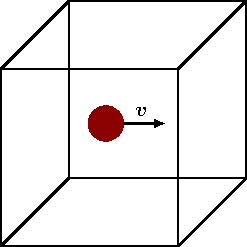
\includegraphics[width=0.8\textwidth]{fig/fig01.pdf}
            \caption{立方体の中での粒子の運動}
          \end{minipage}
          \begin{minipage}{0.3\textwidth}
            \centering
            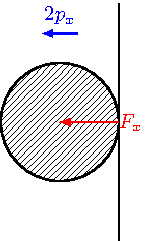
\includegraphics[width=0.8\textwidth]{fig/fig02.pdf}
            \caption{壁に衝突する瞬間}
          \end{minipage}
        \end{figure}

        ここで、$\gamma\equiv1/\sqrt{1-(v/c)^2}$とおけば
        \begin{equation}
          p
          =
          \gamma mv
          \ 、\quad
          E
          =
          \gamma mc^2
        \end{equation}
        なので、$p=Ev/c^2$である。よって
        \begin{graybox}
          \begin{equation}
            \bar{P}
            =
            \frac{1}{3}\cdot\frac{Ev}{c^2}\cdot v
            =
            \frac{Ev^2}{3c^2}
          \end{equation}
        \end{graybox}
        である。また、$m=0$のときは、$E^2=m^2c^4+p^2c^2$から$E=cp$であり$v=c$。ゆえに
        \begin{graybox}
          \begin{equation}
            \bar{P}
            =
            \frac{1}{3}cp
          \end{equation}
        \end{graybox}
        である。


  \item
        エネルギー密度は
        \begin{equation}
          \varepsilon
          =
          g_{*}\int\frac{\dd^3\bm{p}}{(2\pi\hbar)^3}E(\bm{p})f(\bm{p})
        \end{equation}
        なので、$w$は
        \begin{equation}
          w
          =
          \dfrac{\displaystyle
            \int\dd^3\bm{p}\ \dfrac{c^2\bm{p}^2}{3E(\bm{p})}f(\bm{p})
          }{\displaystyle
            \int\dd^3\bm{p}\ E(\bm{p})f(\bm{p})
          }
        \end{equation}
        で与えられる。

        ここで、現在は非相対論的粒子を考えていることから、$E(\bm{p})=mc^2+\bm{p}^2/2m$となる。このとき、粒子の分布$f(\bm{p})$は
        \begin{equation}
          f(\bm{p})
          =
          \left\{ \exp\left[ \dfrac{mc^2+\bm{p}^2/2m-\mu}{k_{\textrm{B}}T} \right] \pm 1 \right\}^{-1}
          \sim
          \exp\left[ -\dfrac{mc^2+\bm{p}^2/2m}{k_{\textrm{B}}T} \right]
        \end{equation}
        となる。ここで、$|\bm{p}|$が大きい領域では$f(\bm{p})\ll 1$であるので、この領域では積分は影響を与えず、つまり$|\bm{p}|\sim 0$付近で評価してよいことが分かる。よって、$E(\bm{p})\sim mc^2,\ \bm{p}^2\sim\varepsilon^2$として
        \begin{graybox}
          \begin{equation}
            w
            \sim
            \frac{c^2\varepsilon^2}{3m^2c^4}
            \sim
            \frac{\varepsilon^2}{m^2}\cdot
            c^{-2}\ll 1
          \end{equation}          
        \end{graybox}
        が得られる。


  \item
        以下の2つの方程式が与えられている:
        \begin{gather}
          \dot{\varepsilon}_{\textrm{DE}}
          +
          3H(1+w_{\textrm{DE}})\varepsilon_{\textrm{DE}}
          =
          0
          、
          \label{eqn:continu}
          \\
          H^2
          =
          \frac{8\pi G}{3c^2}\varepsilon_{\textrm{DE}}
          。
          \label{eqn:freedman}
        \end{gather}
        \eqref{eqn:freedman}を微分すると
        \begin{equation}
          2H\dot{H}
          =
          \frac{8\pi G}{3c^2}\dot{\varepsilon}_{\textrm{DE}}
        \end{equation}
        となるので、\eqref{eqn:continu}を代入し、$\varepsilon_{\textrm{DE}}$に対して\eqref{eqn:freedman}を代入して整理すれば
        \begin{equation}
          \dv{}{t}H
          =
          -\frac{3}{2}(1+w_{\textrm{DE}})H^2
        \end{equation}
        となる。これを$H(t_{0})=H_{0}$のもとで解くと
        \begin{equation}
          \frac{1}{H(t)}
          -
          \frac{1}{H_{0}}
          =
          \frac{3}{2}(1+w_{\textrm{DE}})(t-t_{0})
        \end{equation}
        となる。$\dot{H}=\dot{a}/a$を代入して整理すると
        \begin{equation}
          \frac{1}{a}\dv{a}{t}
          =
          \dfrac{1}{\dfrac{3}{2}(1+w_{\textrm{DE}})(t-t_{0})+\dfrac{1}{H_{0}}}
          。
        \end{equation}
        この常微分方程式の解は
        \begin{graybox}
          \begin{equation}
            a(t)
            =
            a_{0}
            \left[
              \frac{3}{2}H_{0}(1+w_{\textrm{DE}})(t-t_{0})+1
            \right]^{2/3(1+w_{\textrm{DE}})}
          \end{equation}
        \end{graybox}
        である。ただし、$a_{0}\equiv a(t_{0})$とおいた。このとき、$H(t)$の発散が起こるのは$a(t)=0$のときであり、それは
        \begin{graybox}
          \begin{equation}
            t^{\prime}
            =
            t_{0}-\frac{1}{H_{0}(1+w_{\textrm{DE}})}
          \end{equation}          
        \end{graybox}
        であり、$H_{0}=1/145$、$t_{0}=145$を代入すると$t^{\prime}=870\ \textrm{億年}$である。

        \begin{figure}[ht]
          \centering
          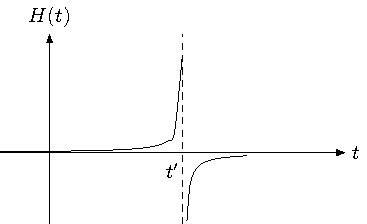
\includegraphics[width=0.6\textwidth]{fig/fig03.pdf}
          \caption{$H(t)$の$t$依存性}
        \end{figure}

\end{enumerate}

\end{document}
